\chapter{Description and gaseous flow validation}
	\label{ch7:bimer_test_bench_and_aero}

\section{Introduction}

Part II has been devoted to the development of models for lagrangian injection. The modeling methodology has been detailed in Chapter \ref{ch4:sli_development}. In a first approach, the models have been constructed from resolved atomization simulations of a liquid jet in crossflow in Chapter \ref{ch5:jicf_resolved_simulations}. Then, the built models have been applied to perform dispersed phase simulations of the same configuration in Chapter \ref{ch6:jicf_lgs_simulations}. The next chapters show the application of the models to a swirled MSFI burner more representative of industrial systems. The same rationale as in Part II is followed: models for lagrangian injection are built from resolved atomization simulations of one multipoint injector hole (Chapter \ref{ch8:bimer_resolved_atomization}), and then applied to initialise dispersed phase simulations of the full take-off stage (Chapter \ref{ch9:BIMER_lagrangian}). 

Prior to the application of the models, this chapter introduces the experimental test bench and the numerical setup replicating this geometry. Non-reactive simulations of the aerodynamic flow field without liquid injection are reported and validated with experiments. Two experimental operating points are simulated: one studied in the thesis of \citeColor[providakis_etude_2013] for validating the numerical simulations, and another one studied by \citeColor[renaud_high-speed_2015] that settles the gaseous field and initial conditions for performing the two-phase flow studies from Chapters \ref{ch8:bimer_resolved_atomization} and \ref{ch9:BIMER_lagrangian}.


\section{Experimental setup}

Banc à Injection Multiple pour les Ecoulements Réactifs (BIMER) is a test rig developed at the laboratory EM2C for the study of reactive phenomena in MSFI systems. Originally studied experimentally by \citeColor[barbosa_etude_2008] with gaseous fuel, its was later extended to liquid fuel in the works of \citeColor[providakis_etude_2013] and \citeColor[renaud_high-speed_2015].

The test bench is shown in Figure \ref{fig:BIMER_test_bench_expe_maquette}. Air is introduced into a cylindrical plenum where the MSFI burner is located. The injector is then connected to a combustion chamber with a length of $500$ mm and a rectangular cross section 150x150 mm$^2$. The lateral walls are made of quartz to allow for optical access to the interior, while the top and bottom walls are cooled with water. Exhaust gases are evacuated at the end of the chamber through a collector. Two different fuel feeding lines are connected to each stage of the injector. A detailed view of the burner is shown in Figure \ref{fig:BIMER_swirler}. Each stage has a swirler and a liquid injector. The swirlers will give a rotating motion to the air coming from the plenum. The stages are designed as follows:

\begin{itemize}

	\item The \textbf{pilot stage} consists of a swirler with 18 vanes located in a crown with inner and outer diameters of 30 and 45 mm respectively. These vanes have a width of 6 mm and a 42$\degree$ inclination angle. Fuel injected through the pilot forms a hollow cone.
	
	\item The \textbf{take-off stage} consists of a swirler with 20 vanes of 35$\degree$ inclination and 10 mm width spanning between inner and outer diameters of 55 and 75 mm. The swirl number generated is close to 1. For liquid injection, 10 holes of $0.3$ mm diameter are equally spaced along the multipoint annulus, with the same radial distance to the center of the pilot injector. Each hole is aligned with the center of a vane (one hole every two vanes), and the vanes are placed so that the swirls of each stage are co-rotating.

\end{itemize}

\begin{figure}[h!]
	\centering
	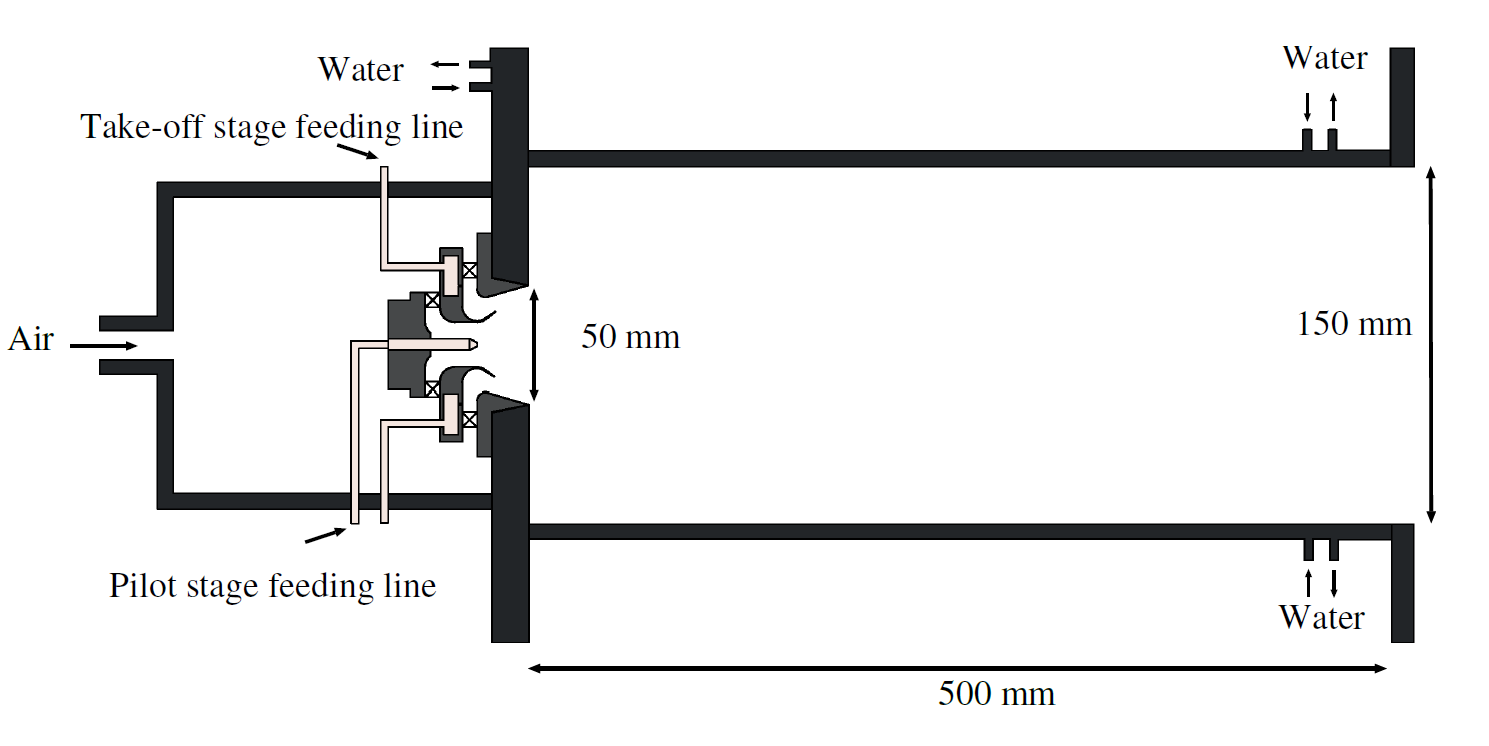
\includegraphics[scale=0.35]{./part3_applications/figures_ch7_aero/BIMER_test_bench_expe_maquette}
	\caption[BIMER experimental test bench]{BIMER experimental test bench. Source: \citeColor[cheneau_etude_2019].}
	\label{fig:BIMER_test_bench_expe_maquette}
\end{figure}

\begin{figure}[h!]
	\centering
	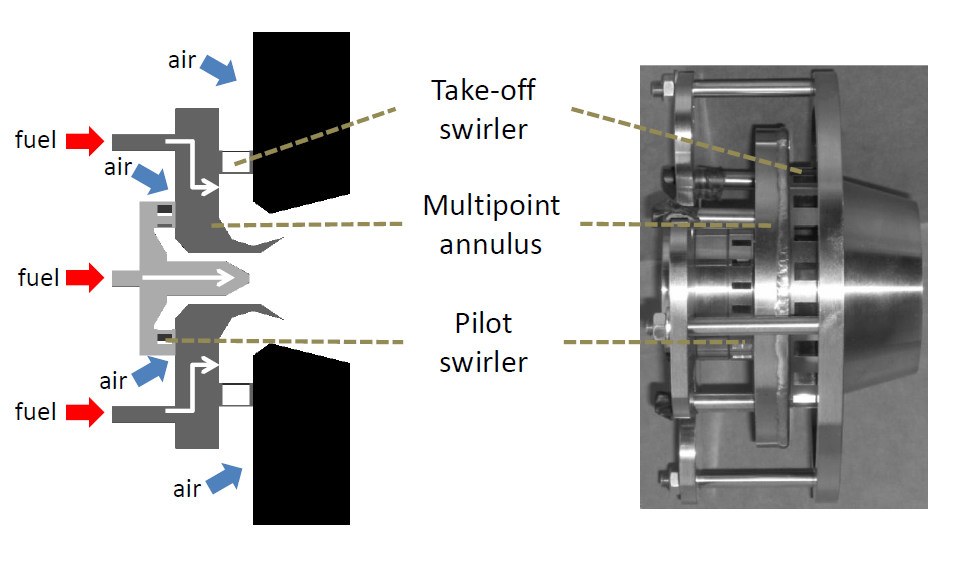
\includegraphics[scale=0.5]{./part3_applications/figures_ch7_aero/BIMER_swirler}
	\caption[Swirled injector of the BIMER test bench]{Swirled injector of the BIMER test bench. \textsl{Left}: schematic cross-section of the injector, indicating air and liquid inlets. \textsl{Right}: experimental view of the injector. Source: \citeColor[renaud_high-speed_2015].}
	\label{fig:BIMER_swirler}
\end{figure}

BIMER is a multi-staged injector where fuel is introduced through both multi-point and pilot stages. The fuel repartition between stages can be defined by the staging parameter $\alpha$, which indicates the quantity of fuel going through the pilot stage $\dot{m}_{l,\mathrm{pilot}}$ with respect to the total fuel:

\begin{equation}
\label{eq:BIMER_staging_parameter}
\alpha = \frac{\dot{m}_{l,\mathrm{pilot}}}{\dot{m}_{l,\mathrm{pilot}} + \dot{m}_{l,\mathrm{takeoff}}}
\end{equation}

where $\dot{m}_{l,\mathrm{takeoff}}$ is the fuel mass flow rate going through the take-off stage. A factor $\alpha = 0 ~\%$ indicates that fuel is injected only through the take-off stage, while $\alpha = 100 ~\%$ denotes pilot injection only. \\

The test bench operates at atmospheric pressure. Air can be preheated up to a temperature of $600$ K. The injected fuel is dodecane. Kerosene is not used since at a laboraty scale it can present risk of coking and its complex chemistry hinders the analysis of the flames \citepColor[providakis_etude_2013]. Hence, dodecane was chosen due to its more simple composition and to its properties being close to kerosene. Dodecane properties of interest for this work are shown in Table \ref{tab:dodecane_properties}.

\begin{table}[!h]
\centering
\caption{Physical properties of dodecane fuel (C$_{12}$H$_26$) at 20 $\degree$C}
\begin{tabular}{ccc}
\thickhline
$\rho$ [kg m$^{-3}$]   & $\mu$ [Pa s]   & $\sigma$ [N m$^{-1}$]  \\
\hline
750 & $1.36 \cdot 10^{-3}$ & 0.022 \\
\thickhline
\end{tabular}
\label{tab:dodecane_properties}
\end{table}

\clearpage

\section{Choice of operating points}

Gaseous flow simulations of BIMER have been performed for two operating conditions tested experimentally \citemColor[providakis_etude_2013,renaud_high-speed_2015]. One condition is used for validation of the aerodynamic simulations, while the other is used as application to obtain a developed gaseous field for initialising two-phase computations in the next chapters:

\begin{itemize}

	\item \textbf{Validation} of the gaseous simulations is performed with the operating point tested experimentally by \citeColor[providakis_etude_2013], since this one presents data on the non-reactive aerodynamic field. The simulations are also compared to numerical results obtained for this same operating condition by \citeColor[cheneau_etude_2019]. 
	
	\item \textbf{Application} to the setup condition tested by \citeColor[renaud_high-speed_2015]. This study shows data on non-reactive spray characteristics, and hence it will be used as the application case to run the full flowchart formerly introduced in Chapter \ref{ch4:sli_development}. %It is, however, not used for validating the gaseous simulations since it does not present pertinent data.

\end{itemize}

The parameters corresponding to both operating points are listed in Table \ref{tab:gaseous_operating_points_BIMER}. 
\begin{table}[!h]
\centering
\caption{Operating points for performing non-reactive gaseous simulations}
\begin{tabular}{ccccccc}
\thickhline
Operating condition    & $\dot{m}_g$ [g s$^{-1}$] & $T_g$ [K] & $\rho_g$ [kg m$^{-3}]$  & $\mu_g$ [Pa s] & $p$ [atm]  & Reference\\
\hline
Validation &   53 & 473 & 0.75 & $2.57 \cdot 10^{-5}$ & 1 & \citeColor[providakis_etude_2013]\\
Application  & 43.1 & 433 & 0.82 & $2.39 \cdot 10^{-5}$ & 1 & \citeColor[renaud_high-speed_2015] \\
%Validation &   53 & 473 & 0.746089 & $2.571 \cdot 10^{-5}$ & 1 & \citeColor[providakis_etude_2013]\\
%Application  & 43.1 & 433 & 0.816382 & $2.391 \cdot 10^{-5}$ & 1 & \citeColor[renaud_high-speed_2015] \\
\thickhline
\end{tabular}
\label{tab:gaseous_operating_points_BIMER}
\end{table}



\section{Numerical setup}


\subsection{Computational geometry}

The computational configuration of the BIMER test bench is shown in Figure \ref{fig:BIMER_geometry_full_domain}. Air is introduced into the plenum through a cylindrical nozzle. The MSFI burner is located at the end of the plenum. A diffusor connects the burner to the combustion chamber. At the end of the chamber, a region representing the atmosphere is located with a coflow of air at low speed ($5$ m/s). 

\begin{figure}[h!]
	\centering
	\includeinkscape[inkscapelatex=false,scale=0.25]{./part3_applications/figures_ch7_aero/BIMER_geometry_full_domain}
	\caption{Numerical configuration of BIMER test bench}
	\label{fig:BIMER_geometry_full_domain}
\end{figure}

Figure \ref{fig:BIMER_geometry_flower_details} gives a detailed view of the MSFI burner. Both the take-off and pilot stages are represented as in the experimental geometry, with the fuel injectors and the gaseous swirlers. Fuel feeding lines and other experimental features have not been modeled due to their geometrical complexity \citepColor[cheneau_etude_2019]. The flower, whose main function is to fix the burner to the test rig, has been included in the computational domain since it influences the incoming gaseous flow field.

\begin{figure}[h!]
	\centering
	\includeinkscape[inkscapelatex=false,scale=0.25]{./part3_applications/figures_ch7_aero/BIMER_geometry_flower_details}
	\caption[Details of multipoint injector from BIMER test bench.]{Details of multipoint injector from BIMER test bench. \textsl{Left}: side view indicating same features of Figure \ref{fig:BIMER_swirler}. \textsl{Right}: isometric view of the injector, with a zoom-in region showing the multipoint injector.}
	\label{fig:BIMER_geometry_flower_details}
\end{figure}

\subsection{Meshes}

For the numerical gaseous study of BIMER, two meshes have been simulated. Their characteristics are given in Table \ref{tab:BIMER_meshes_gaseous}: a grid independence study has been performed with a coarse mesh of $5$ million elements and a fine one of $38$ million elements. 

\begin{table}[!h]
\centering
\caption{Characteristics of meshes employed in BIMER study}
\begin{tabular}{ccccccc}
\thickhline
Mesh   & $\#$ elements & $\#$ nodes & Minimum cell size $\Delta x$ [$\mu$m] \\
\hline
%Coarse & 5,200,992 & 932,974 & & &  \\
Coarse & 7,356,140 & 1,891,542 & 29.82 \\ % $\Delta t = 1$ [$\mu$s]
Fine & 37,835,617 & 9,738,371 & 5.04\\ % $\Delta t = 0.5$ [$\mu$s]
\thickhline
\end{tabular}
\label{tab:BIMER_meshes_gaseous}
\end{table}

%Figure \ref{fig:BIMER_meshes} provides a view of both meshes, with zoomed-in views of the injector where both meshes are refined. At the plenum, the baseline cell size is $\Delta x = 3$ mm for both meshes. Then, for the coarse mesh the injector region is refined overall with $\Delta x = 1.7$ mm. Further downstream, along the combustion chamber the cell size evolves gradually from $\Delta x = 3$ mm at the exit of the injector until $\Delta x = 8$ mm at the inlet of the atmospheric region. The injector walls are not refined in this case. For the fine mesh, on the contrary, the injector overall mesh size is $\Delta x = 0.5$ mm. The walls of the pilot and take-off have been refined to $\Delta x = 0.25$ mm. At the exit of the injector, a conic region has been placed with a baseline size of $\Delta x = 1$ mm. Further downstream the combustion chamber, the cell size evolves from this value until $\Delta x = 8$ mm at the inlet of the atmospheric region as in the coarse mesh.

Figure \ref{fig:BIMER_meshes} provides a view of both grids, with zoomed-in views of the injector where more elements are placed. At the plenum, the baseline cell size is $\Delta x = 3$ mm. Then, the injector region is refined overall with $\Delta x = 0.5$ mm for both meshes. In the coarse mesh, the cell size in the combustion chamber  evolves gradually from $\Delta x = 3$ mm at the exit of the injector until $\Delta x = 8$ mm at the inlet of the atmospheric region. The injector walls are not refined in this case. For the fine mesh, on the contrary, the walls of the pilot and take-off have been refined to $\Delta x = 0.25$ mm. At the exit of the injector, a conic region has been placed with a baseline size of $\Delta x = 1$ mm. Downstream the combustion chamber, the cell size evolves from $\Delta x = 1$ mm to $\Delta x = 8$ mm at the inlet of the atmospheric region as in the coarse mesh. Simulations are run using an LES approach where a dynamic Smagorinsky filter is used to model the subgrid turbulent scales \citepColor[germano_dynamic_1991].

\newpage

\begin{figure}[ht]
\centering
\begin{subfigure}[b]{1.0\textwidth}
	\centering
   \includeinkscape[inkscapelatex=false,scale=0.35]{./part3_applications/figures_ch7_aero/BIMER_mesh_coarse}
   \caption{Coarse mesh}
   \label{fig:BIMER_mesh_fine} 
\end{subfigure}
\begin{subfigure}[b]{1.0\textwidth}
	\centering
   \includeinkscape[inkscapelatex=false,scale=0.35]{./part3_applications/figures_ch7_aero/BIMER_mesh_fine}
   \caption{Fine mesh}
   \label{fig:BIMER_mesh_fine}
\end{subfigure}
\caption{View of the meshes employed for the BIMER study at the central plane of the burner.}
\label{fig:BIMER_meshes}
\end{figure}


\section{Physical features of swirled flows}

\subsection{Swirl number and vortex breakdown}
\label{subsec:BIMER_ch7_sw_vortex_breakdown}

Swirled flows are characterized by a high rotational flow measured by the azimuthal velocity component $u_\theta$. The relative importance of this component with respect to the axial velocity will determine the characteristics of the gaseous flow. This can also be specified by means of the swirl number $S_w$, which is calculated as the ratio between the azimuthal and axial momentum fluxes \citepColor[huang_dynamics_2009]:

\begin{equation}
S_w = \frac{G_\theta}{R_\mathrm{ext} G_x} = \frac{1}{R_\mathrm{ext}} \frac{\int_0^{R_\mathrm{ext}} \rho u u_\theta r^2 dr}{\int_0^{R_\mathrm{ext}} \rho u^2 r dr}
\end{equation}

where $R_\mathrm{ext}$ is the outer radius of injection. For $S_w$ values over a given critical value, usually 0.6 \citepColor[syred_combustion_1974], a phenomenon known as vortex breakdown appears. Vortex breakdown is manifested by the appearance of the recirculation zones and instabilities in the aerodynamic field and in the flame dynamics. A common hydrodynamic instability, present in most swirled burners, is the Precessing Vortex Core (PVC). In the operating points from Table \ref{tab:gaseous_operating_points_BIMER}, the values of $S_w$ are around unity \citemColor[providakis_etude_2013,renaud_high-speed_2015], which are higher than the threshold $S_w > 0.6$. Hence, in both operating conditions the mentioned phenomena are present. The recirculation regions are shown and discussed for both the validation ($\S$\ref{sec:ch7_BIMER_validation_point}) and application points ($\S$\ref{ch7:BIMER_application_point}), while the PVC instability is shown only for the latter.

\subsection{Characteristic time scales}

Characteristic time scales of the gaseous flow field can be estimated from the simulations. Their calculation is based on the mean axial and azimuthal velocities, $\overline{u}_x$ and $\overline{u}_\theta$ respectively. For their obtention, the following expressions are applied at the diffusor outlet:

\begin{equation}
\overline{u}_x \approx \frac{1}{R_d} \int_0^{R_d} u_x dl ~~ ; ~~ \overline{u}_\theta \approx \frac{1}{R_d} \int_0^{R_d} u_\theta dl
\end{equation}

where $R_d = 25$ mm is the diffusor outlet radius. Two time scales are defined: 

\begin{itemize}

	\item Convective time scale $\tau_\mathrm{conv}$:
	
	\begin{equation}
	\tau_\mathrm{conv} = \frac{L_{cc}}{\overline{u}_x} 
	\end{equation}
	
	where $L_{cc} = 500$ mm is the length of the combustion chamber.
	
	\item Swirl time scale $\tau_\mathrm{swirl}$:
	
	\begin{equation}
	\tau_\mathrm{swirl} = \frac{\pi R_d}{\overline{u}_{\scriptsize{\theta}}}
	\end{equation}	
	
\end{itemize}

The mean velocities and time scales are obtained for both operating points simulated. The results are shown in Table \ref{tab:gaseous_field_timescales}.

\begin{table}[!h]
\centering
\caption{Gaseous fields time scales for each operating point}
\begin{tabular}{ccccc}
\thickhline
Operating condition    & $\overline{u}_x$ [m s$^{-1}$]   & $\overline{u}_\theta$ [m s$^{-1}$] & $\tau_\mathrm{conv}$  [ms] &  $\tau_\mathrm{swirl}$ \\
\hline
Validation & 17.1 & 23.3  & 29.2 & 3.4 \\
Application & 13.3 & 18.0 & 37.6 & 4.4 \\
\thickhline
\end{tabular}
\label{tab:gaseous_field_timescales}
\end{table}


\section{Validation of gaseous field}
\label{sec:ch7_BIMER_validation_point}

The numerical setup introduced previously is firstly validated on the corresponding operating from Table \ref{tab:gaseous_operating_points_BIMER}, tested experimentally in \citeColor[providakis_etude_2013]. This point was also numerically studied in the work of \citeColor[cheneau_etude_2019] with a mesh of 20.1 million elements and with the software AVBP, developed at CERFACS \citepColor[cerfacs_avbp_2011] and which uses different numerics to the software YALES2. Details on the mesh and parameters used in this study can be found in the reference previously mentioned. Regarding the results obtained in this work, two computations have run with YALES2 (one with each mesh shown in Figure \ref{fig:BIMER_meshes}) for a total physical time of 180 ms. For flow establishment, simulations have run first for a total physical time of 60 ms ($\sim 2 \tau_{conv}$). At the end of this time, statistics have been accumulated for a physical time of 120 ms ($\sim 4 \tau_{conv}$). All the mean values reported in this section have been time-averaged for this duration.

In first place, the meshes employed are assessed by plotting the ratio between the mean turbulent viscosity and the laminar viscosity $\overline{\nu}_T / \overline{\nu}$ in the central plane. $\overline{\nu}_T$ is the turbulent viscosity modeled by the LES subgrid model, in this case the dynamic Smagorinsky model \citepColor[germano_dynamic_1991]. A dynamic model has been chosen since it provides values of modelled turbulent viscosity lower than the static ones, hence improving the simulation results in recirculation regions and turbulent boundary layers \citepColor[sayadi_comparative_2010]. The results are shown in Figure \ref{fig:BIMER_NU_ratios}. In both meshes, the ratio is high upstream the multipoint injector and low within it, since both meshes have similar characteristics in these regions (see Figure \ref{fig:BIMER_meshes}) except for the wall refinement in the fine mesh, which has not a big impact on the viscosity ratio in this case. The biggest differences are located downstream the injector: the values of the viscosity ratio are much smaller in the fine mesh than in the coarse one due to the reduction in element size. In both meshes, there is a transition of  $\overline{\nu}_T / \overline{\nu}$ in the central plane. $\overline{\nu}_T$ in the divergent section due to a steep gradient in the cell size, which is more pronounced in the coarse case. In general, the lower values of the viscosity ratio in the fine mesh downstream the injector indicate that the turbulent model contributes to a lesser extent, hence improving the LES quality (making it closer to DNS) in these regions for this resolution.


\clearpage

\begin{figure}[ht]
\centering
\begin{subfigure}[b]{0.45\textwidth}
	\centering
   \includeinkscape[inkscapelatex=false,scale=0.32]{./part3_applications/figures_ch7_aero/BIMER_nu_ratio/BIMER_nu_ratio_fine}
   \caption{Fine mesh}
   \label{fig:field_NU_T_NU_mean_fine}
\end{subfigure}
\begin{subfigure}[b]{0.45\textwidth}
	\centering
   \includeinkscape[inkscapelatex=false,scale=0.32]{./part3_applications/figures_ch7_aero/BIMER_nu_ratio/BIMER_nu_ratio_coarse}
   \caption{Coarse mesh}
   \label{fig:field_NU_T_NU_mean_coarse}
\end{subfigure}
\caption[Ratio between turbulent mean viscosity and mean viscosity in central plane]{Ratio between turbulent mean viscosity and mean viscosity in central cut of BIMER.}
\label{fig:BIMER_NU_ratios}
\end{figure}

The mean axial field for in the middle plane is shown in Figure \ref{fig:BIMER_mean_axial_velocities}. The white line indicates the contour with zero mean axial velocity, $\overline{u} = 0$. The results obtained by \citeColor[cheneau_etude_2019] are also shown for comparison. As observed, the range of mean velocity values is the same in the three cases. The flow fields are similar: the topology is typical of swirled burners, containing an Inner Recirculation Zone (IRZ), a Corner Recirculation Zone (CRZ), two Swirled Jets (SWJ) and shear layers with high velocity gradients. These areas are indicated by arrows only in Figure \ref{fig:BIMER_mean_axial_velocities}b, but are present in all the cases. With respect to differences among meshes, the coarse mesh shows a continuous region of negative velocity from the pilot injection point and for the whole domain shown in the figure, while the fine mesh displays a small region of positive velocity between the pilot injector and the tip of the IRZ (stagnation point) as the results of \citeColor[cheneau_etude_2019] show. Furthermore, the SWJ in the coarse mesh show larger numerical diffusion than in the fine case due to the larger cell sizes.

\begin{figure}[ht]
\centering
\begin{subfigure}[b]{0.4\textwidth}
	\centering
   \includeinkscape[inkscapelatex=false,scale=0.32]{./part3_applications/figures_ch7_aero/BIMER_validation_qualitative_mean_field/field_axial_velocity_mean_fine}
   \caption{Results obtained with the fine mesh}
   \label{fig:field_axial_velocity_mean_fine}
\end{subfigure}
\hspace{0.8in}
\begin{subfigure}[b]{0.4\textwidth}
	\centering
   \includeinkscape[inkscapelatex=false,scale=0.32]{./part3_applications/figures_ch7_aero/BIMER_validation_qualitative_mean_field/field_axial_velocity_mean_coarse}
   \caption{Results obtained with the coarse mesh}
   \label{fig:field_axial_velocity_mean_coarse}
\end{subfigure}
\begin{subfigure}[b]{1.0\textwidth}
	\centering
   \includeinkscape[inkscapelatex=false,scale=0.32]{./part3_applications/figures_ch7_aero/BIMER_validation_qualitative_mean_field/field_axial_velocity_mean_cheneau}
   \caption{Results from \citeColor[cheneau_etude_2019].}
   \label{fig:field_axial_velocity_mean_cheneau} 
\end{subfigure}
\caption[Mean axial velocities at central plane in BIMER]{Mean axial velocities at central plane in BIMER. The white line indicates the contour $\overline{u} = 0$.}
\label{fig:BIMER_mean_axial_velocities}
\end{figure}


\clearpage
 
The pictures from Figure \ref{fig:BIMER_mean_axial_velocities} show a qualitative view of the mean axial velocity field from only computational results. The numerical results are now validated by comparing with experimental results obtained with Particle Image Velocimetry (PIV) at the probes shown in Figure \ref{fig:BIMER_mean_axial_velocities}a: a qualitative validation is performed by showing mean and RMS velocity maps in the rectangular section, while quantitative results can be compared by plotting the velocity profiles at the lines located at x = 30, 50 mm downstream the diffusor.

%Results are contained here: $Ongoing - BIMER - postprocessing - aero$. They were discussed in the pilotage of 16 March 2021.

%Show nice streamlines (Fig. 6.4 Esclapez-1) and PVC. It would be nice to compare them for both operating conditions

 % Show mean field (velocities, indicate, IRZ, ORZ, vortical structures ...) for coarse and fine meshes  (see pilotage 2021-03-16).

\vspace{-0.1in}
\subsection{Qualitative validation}

Experimental validation of the simulations with experimental results is done by comparing the velocity maps at the rectangular probe, see Figure \ref{fig:validation_qualitative_velocity_fields}. The experimental fields from \citeColor[providakis_etude_2013] are shown in the first column, while the numerical results from \citeColor[cheneau_etude_2019] obtained with the software AVBP are located in the second one. Mean and RMS axial and vertical velocities are depicted. The black lines denote the contours of zero mean axial velocity, $\overline{u} = 0$.

The results obtained with both fine and coarse meshes show a good flow topology in all cases. The velocities are in the same range as the experiments, with some over(under)estimation of the maximum (minimum) values in the computations. The lines of null axial velocity are properly reproduced in both fine and coarse meshes, with differences in the CRZ probably due to the non-convergence in this regions: these are low-velocity, recirculation areas which take longer to converge than other parts of the domain, and hence the running time of the simulations might not be enough to fully resolve them. 

With respect to the axial velocities $u$, the mean maps from Figure \ref{fig:validation_qualitative_velocity_fields}a show that both IRZ and CRZ are well captured. The shear layers between IRZ and CRZ, where the velocity gradients are high, are also resolved. Symmetry with respect to the central axis is observed. For $u_\mathrm{RMS}$ (Figure \ref{fig:validation_qualitative_velocity_fields}b), symmetry with respect to this line is also observed. The RMS values are higher at the IRZ and the shear layers, where high velocity fluctuations are present. In general, RMS values are overestimated in the simulations with respect to the experiments. With respect to the vertical velocities $v$, the mean values from Figure \ref{fig:validation_qualitative_velocity_fields}c far downstream the diffusor match the experiments. Closer, the simulations present two circular pockets of high positive and negative velocities (enclosed by the dashed contours in Figure \ref{fig:validation_qualitative_velocity_fields}c, fine case) that are not present in the experiments. The $v_\mathrm{RMS}$ values of Figure \ref{fig:validation_qualitative_velocity_fields}d do not fully agree with the experiments. The experimental results for the mean velocity, however, do not present symmetry with respect to the central axis, something which is expected in this type of swirled configurations. Overall, all the numerical results obtained with both fine and coarse meshes match closely the numerical results obtained with AVBP by \citeColor[cheneau_etude_2019].

By comparing the results from both fine and coarse meshes, it is observed that both meshes provide values with the same order of magnitude for all velocities. The RMS values obtained with the coarse mesh are lower than for the fine one. Also, it is clearly seen that the fields obtained with the fine mesh are smoother (i.e. present less numerical noise) than the ones with the coarse one. This is attributed to numerical diffusion in the simulations, which is higher for the coarse mesh. The diffusion is more noticeable in the regions with high velocity gradients such as the shear layers of $\overline{u}$ and the velocity pockets of $\overline{v}$, where the numerical noise in the velocity field is visible. 

\vspace{-0.1in}
\subsection{Quantitative validation}

The qualitative analyses are complemented with a qualitative experimental validation by showing the velocity profiles at the lines x = 30, 50 mm displayed in Figure \ref{fig:field_axial_velocity_mean_fine}.  The results are shown in Figure \ref{fig:BIMER_quantitative_validation_axial_velocities} for the axial velocities $u$ and Figure \ref{fig:BIMER_quantitative_validation_verticals_velocities} for the vertical ones, $v$. Once again, the experimental results by \citeColor[providakis_etude_2013] and the numerical ones by \citeColor[cheneau_etude_2019] are also shown. The location of maxima and minima peaks in mean velocities are properly captured. Their magnitudes are overestimated in absolute value for $\overline{u}$ at x = 30 mm, while they get closer to the experimental results at x = 50 mm. The RMS values are always overestimated in the simulations, specially in the regions with higher velocity gradients, as also shown in the qualitative images of Figure \ref{fig:validation_qualitative_velocity_fields}. The comparison for the vertical velocities does not fully match the experimental results, but it agrees with the numerical results obtained with AVBP by  \citeColor[cheneau_etude_2019]. In general, all results show symmetry with the central axis x = 0.

By comparing the results from the fine and coarse meshes, the same statements as in the previous section for the qualitative validation can be done. The coarse mesh presents noisier signals due to the higher numerical diffusion introduced in this case. The mean values for the axial velocity $\overline{u}$ are quite close in both cases, but the difference is larger for the vertical velocity $\overline{v}$. The RMS values in the coarse mesh are generally underestimated along the $z$ coordinate. Due to the better results obtained with the fine mesh, this case is retrieved for simulating the application point described in Figure \ref{tab:gaseous_operating_points_BIMER} (see $\S$\ref{ch7:BIMER_application_point}) and for performing the subsequents computations shown in Chapters \ref{ch8:bimer_resolved_atomization} and \ref{ch9:BIMER_lagrangian}.


\clearpage

\begin{figure}[h!]
\centering
\begin{subfigure}[b]{1.0\textwidth}
	\centering
	 \includeinkscape[inkscapelatex=false,scale=0.23]{./part3_applications/figures_ch7_aero/BIMER_validation_qualitative_maps/u_mean}
   \caption{Mean axial velocity}
   \label{fig:validation_qualitative_u_mean} 
\end{subfigure}
\begin{subfigure}[b]{1.0\textwidth}
	\centering
	 \includeinkscape[inkscapelatex=false,scale=0.23]{./part3_applications/figures_ch7_aero/BIMER_validation_qualitative_maps/u_rms}
   \caption{RMS axial velocity}
   \label{fig:validation_qualitative_u_rms}
\end{subfigure}
\begin{subfigure}[b]{1.0\textwidth}
	\centering
	 \includeinkscape[inkscapelatex=false,scale=0.23]{./part3_applications/figures_ch7_aero/BIMER_validation_qualitative_maps/v_mean}
   \caption{Mean vertical velocity}
   \label{fig:validation_qualitative_v_mean} 
\end{subfigure}
\begin{subfigure}[b]{1.0\textwidth}
	\centering
	 \includeinkscape[inkscapelatex=false,scale=0.23]{./part3_applications/figures_ch7_aero/BIMER_validation_qualitative_maps/v_rms}
   \caption{RMS vertical velocity}
   \label{fig:validation_qualitative_v_rms}
\end{subfigure}
\caption[Qualitative experimental validation]{Qualitative experimental validation: velocity fields in enclosed region from Figure \ref{fig:field_axial_velocity_mean_fine}. The first column denotes the experimental results by \citeColor[providakis_etude_2013], and the second one the numerical results obtained with AVBP by \citeColor[cheneau_etude_2019].}
\label{fig:validation_qualitative_velocity_fields}
\end{figure}


\clearpage

\begin{figure}[h!]
\centering
\begin{subfigure}[b]{0.22\textwidth}
	\centering
   \includegraphics[scale=0.25]{./part3_applications/figures_ch7_aero/BIMER_validation_quantitative_lines/x30_u_axial_mean.eps} 
   %\caption{Case UG100\_DX20: crossflow planes}
   %\label{} 
\end{subfigure}
   \hspace{0.05in}
\begin{subfigure}[b]{0.22\textwidth}
	\centering
   \includegraphics[scale=0.25]{./part3_applications/figures_ch7_aero/BIMER_validation_quantitative_lines/x30_u_axial_rms.eps} 
   %\caption{Case UG100\_DX20: filming planes}
   %\label{}
\end{subfigure}
\hfill
%\vskip\baselineskip
\begin{subfigure}[b]{0.22\textwidth}
	\centering
   \includegraphics[scale=0.25]{./part3_applications/figures_ch7_aero/BIMER_validation_quantitative_lines/x50_u_axial_mean.eps} 
   %\caption{Case UG100\_DX10: crossflow planes}
   %\label{} 
\end{subfigure}
   \hspace{0.05in}
\begin{subfigure}[b]{0.22\textwidth}
	\centering
   \includegraphics[scale=0.25]{./part3_applications/figures_ch7_aero/BIMER_validation_quantitative_lines/x50_u_axial_rms.eps}
   %\caption{Case UG100\_DX10: filming planes}
   %\label{}
\end{subfigure}
\caption{Mean and RMS axial velocity profiles along probes lines at x = 30, 50 mm.}
\label{fig:BIMER_quantitative_validation_axial_velocities}
\end{figure}



\begin{figure}[h!]
\centering
\begin{subfigure}[b]{0.22\textwidth}
	\centering
   \includegraphics[scale=0.25]{./part3_applications/figures_ch7_aero/BIMER_validation_quantitative_lines/x30_w_vertical_mean.eps} 
   %\caption{Case UG100\_DX20: crossflow planes}
   %\label{} 
\end{subfigure}
   \hspace{0.05in}
\begin{subfigure}[b]{0.22\textwidth}
	\centering
   \includegraphics[scale=0.25]{./part3_applications/figures_ch7_aero/BIMER_validation_quantitative_lines/x30_w_vertical_rms.eps} 
   %\caption{Case UG100\_DX20: filming planes}
   %\label{}
\end{subfigure}
\hfill
%\vskip\baselineskip
\begin{subfigure}[b]{0.22\textwidth}
	\centering
   \includegraphics[scale=0.25]{./part3_applications/figures_ch7_aero/BIMER_validation_quantitative_lines/x50_w_vertical_mean.eps} 
   %\caption{Case UG100\_DX10: crossflow planes}
   %\label{} 
\end{subfigure}
   \hspace{0.05in}
\begin{subfigure}[b]{0.22\textwidth}
	\centering
   \includegraphics[scale=0.25]{./part3_applications/figures_ch7_aero/BIMER_validation_quantitative_lines/x50_w_vertical_rms.eps}
   %\caption{Case UG100\_DX10: filming planes}
   %\label{}
\end{subfigure}
\caption{Mean and RMS vertical velocity profiles along probes lines at x = 30, 50 mm.}
\label{fig:BIMER_quantitative_validation_verticals_velocities}
\end{figure}


\clearpage

\section{Application point}
	\label{ch7:BIMER_application_point}
	
According to the results obtained for the validation point, the application point from Table \ref{tab:gaseous_operating_points_BIMER} is simulated with the fine mesh shown in Figure \ref{fig:BIMER_meshes}. In this case, the application point has been run for a total physical time of 240 ms: 80 ms ($\sim 2 \tau_{conv}$) for flow establishment, and then statistics have been accumulated for 160 ms ($\sim 4 \tau_{conv}$). These values have been chosen to keep the same convergence time with respect to the convective characteristic time as in the validation point.
	
Figure \ref{fig:BIMER_application_streamlines} shows the mean axial velocity field $\overline{u}$ with the streamlines (black contours). The contours of null mean axial velocity $\overline{u} = 0$ are also shown (white lines). The IRZ and ORZ recirculation zones are clearly observed, as well as SWJ branches and the shear layers. As in the validation point (Figure \ref{fig:BIMER_mean_axial_velocities}), the flow field is typical of gaseous swirled jets for values of $S_w \approx 1$. A stagnation point in the tip of the IRZ, closer to the pilot injector, is also observed. The magnitudes of mean axial velocity are larger than in the application case since the injected mass flow rate is lower.

\begin{figure}[ht]
\centering
\includeinkscape[inkscapelatex=false,scale=0.5]{./part3_applications/figures_ch7_aero/BIMER_application_U/application_streamlines_and_U_mean}
\caption[Streamlines and mean axial velocity field for the application point of BIMER]{Streamlines and mean axial velocity field for the application point of BIMER. The while line indicates the iso-contour of $\overline{u} = 0$.}
\label{fig:BIMER_application_streamlines}
\end{figure}

\subsection{Velocity fields in the middle plane}

The mean and RMS velocity fields in the axial, vertical and transversal directions are shown in Figure \ref{fig:field_application}. The high values of mean vertical velocity $\overline{v}$ in the diffusor indicate the jet opening, and can influence the fuel introduced through the multipoint injector: as shown later in Chapter \ref{ch9:BIMER_lagrangian}, such high velocities make the injected spray to open and approach the walls of the diffusor, while moving away from the central line $x = 0$. This creates a \textsl{hollow cone} of droplets if the pilot injector is not activated. Furthermore, the mean transversal velocity $\overline{w}$ has also a very strong component, which will give a rotational motion to the droplets in the azimuthal direction. The high maximum values of $\overline{w}$, which are of the order of $\overline{u}$, indicate a strong swirl of the jet, being in accord with the value for the swirl number $S_w \sim 1$ as stated by \citeColor[renaud_high-speed_2015].

In all cases, the RMS values are really high closer to the injector and decrease further downstream. In the axial velocity field, the highest values are located in the divergent section of the pilot nozzle, probably due to flow detachment in this region.  For the vertical and transversal velocities, the highest RMS are found between the pilot injector tip and the stagnation point of the IRZ. This indicates high velocity fluctuations in this region, which can have a strong influence on the spray injected through the pilot nozzle. The fact that the magnitude of the RMS are of the same order as the mean values indicates a highly turbulent flow. 


\clearpage


\begin{figure}[ht]
\centering
\begin{subfigure}[b]{1.0\textwidth}
	\centering
   \includeinkscape[inkscapelatex=false,scale=0.9]{./part3_applications/figures_ch7_aero/BIMER_application_U/field_U_axial_velocity}
   \caption{Axial velocity $u$}
   \label{fig:field_application_axial_velocity}
\end{subfigure}
%\vskip\baselineskip
\begin{subfigure}[b]{1.0\textwidth}
	\centering
   \includeinkscape[inkscapelatex=false,scale=0.9]{./part3_applications/figures_ch7_aero/BIMER_application_U/field_V_vertical_velocity}
   \caption{Vertical velocity $v$}
   \label{fig:field_application_vertical_velocity}
\end{subfigure}
%\vskip\baselineskip
\begin{subfigure}[b]{1.0\textwidth}
	\centering
   \includeinkscape[inkscapelatex=false,scale=0.9]{./part3_applications/figures_ch7_aero/BIMER_application_U/field_W_transversal_velocity}
   \caption{Transversal velocity $w$}
   \label{fig:field_application_transversal_velocity} 
\end{subfigure}
\caption[Mean and RMS velocity fields at central plane in BIMER for the application point]{Mean and RMS velocity fields at central plane in BIMER for the application point.}
\label{fig:field_application}
\end{figure}

\clearpage

\subsection{Turbulent structures}

As specified in $\S$\ref{subsec:BIMER_ch7_sw_vortex_breakdown}, when $S_w > 0.6$ a change in the flow field topology due to the strong rotational motion appears, known as vortex breakdown \citepColor[lucca-negro_vortex_2001]. This topology change creates two main features: different recirculation regions, discussed previously and seen in Figures \ref{fig:BIMER_mean_axial_velocities} and \ref{fig:BIMER_application_streamlines}, and the appearance of the Precessing Vortex Core (PVC). The PVC is a helical structure of high rotational velocity arising from an instability in the shear layer at the exit of the injector. It rotates around the axis of symmetry. Figure \ref{fig:BIMER_application_turbulent_structures} left shows the PVC visualized by a isobaric contour of low static pressure. The PVC can strongly impact the spray dispersion and the mixing field in reactive cases, creating pockets of low mixture fraction where ignition could hardly take place \citepColor[jaegle_eulerian_2011].

Finally, the high turbulent state found within BIMER can also be demonstrated by showing the unsteady, coherent vortical structures of the flow. Such structures can be illustrated with the Q-criterion defined by \citeColor[jeong_identification_1995]:

\begin{equation}
Q = \frac{1}{2} \left( \Omega_{ij} \Omega_{ij} - S_{ij} S_{ij} \right)
\end{equation}

where $\Omega_{ij} = \frac{1}{2} \left( \frac{\partial u_i}{\partial x_j} - \frac{\partial u_j}{\partial x_i} \right)$ and $S_{ij} = \frac{1}{2} \left( \frac{\partial u_i}{\partial x_j} + \frac{\partial u_j}{\partial x_i} \right)$ are respectively the symmetric and antisymmetric components of $\nabla \textbf{u}$. Figure \ref{fig:BIMER_application_turbulent_structures} right shows the vortical structures visualized through an iso-contour Q = $2 \cdot 10^8$ s$^{-2}$. Small eddies are created at the exit of the injector, upstream the diffuser, due to the swirling motion of the flow. Further downstream, the eddies show larger characteristic sizes. These vortices show a transversal structure and more wrinkling with respect to the vortices upstream, probably due to the roll-up of shear layers in this region \citepColor[huang_systematic_2006].

%\begin{equation}
%S_{ij} = \frac{1}{2} \left( \frac{\partial u_i}{\partial x_j} + \frac{\partial u_j}{\partial x_i} \right) ~~~~ ; ~~~~ \Omega_{ij} = \frac{1}{2} \left( \frac{\partial u_i}{\partial x_j} - \frac{\partial u_j}{\partial x_i} \right)
%\end{equation}




% ref vortices in swirl: https://arc.aiaa.org/doi/pdf/10.2514/1.15382

\begin{figure}[ht]
\centering
\begin{subfigure}[b]{0.4\textwidth}
	\centering
   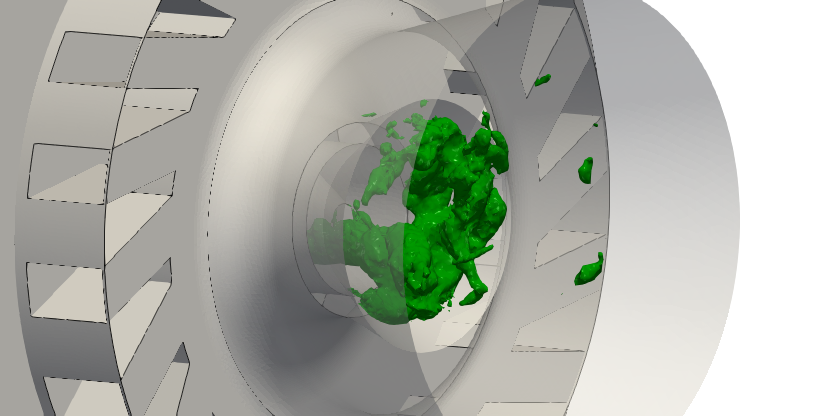
\includegraphics[scale=0.35]{./part3_applications/figures_ch7_aero/BIMER_application_PVC/PVC_P_m3000}
   %\caption{PVC visualization (green) by iso-contour of statis pressure}
   \label{fig:BIMER_application_PVC}
\end{subfigure}
\hspace{0.8in}
\begin{subfigure}[b]{0.4\textwidth}
\centering
   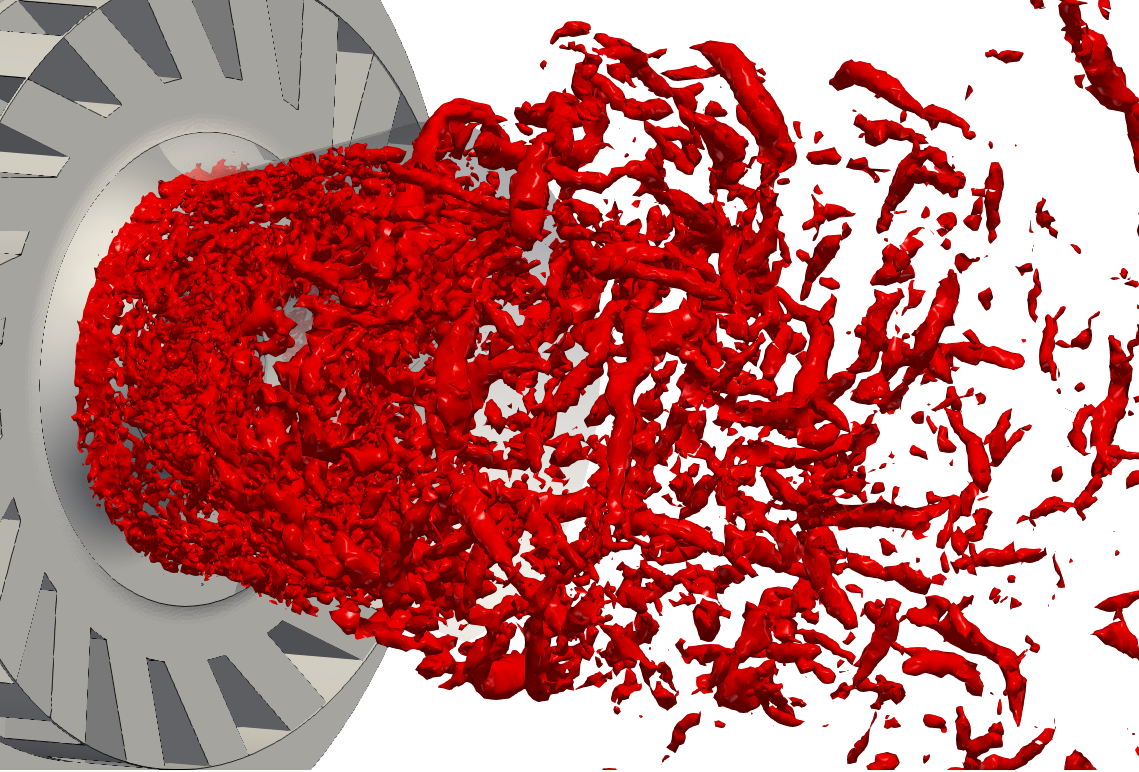
\includegraphics[scale=0.35]{./part3_applications/figures_ch7_aero/BIMER_application_PVC/Q_crit_2e8}
   %\caption{Vortical structures shown by iso-surface of Q-criterion}
   \label{fig:BIMER_application_Qcrit}
\end{subfigure}
\caption[Turbulent structures in BIMER]{Turbulent structures in BIMER. \textsl{Left}: PVC visualization (blue) by iso-contour of static pressure. \textsl{Right}: Vortical structures (red) shown by iso-surface of Q-criterion}
\label{fig:BIMER_application_turbulent_structures}
\end{figure}






\section{Conclusion}

This chapter has presented non-reactive LES gaseous simulations of the BIMER test bench. In first place, the experimental test rig at EM2C and the operating conditions chosen to perform simulations have been introduced. Two experimental points have been chosen: one studied by \citeColor[providakis_etude_2013] to validate the simulations and numerical setup, since it presents qualitative and quantitative data on the gaseous flow field, and another one tested by \citeColor[renaud_high-speed_2015] which does not show aerodynamic quantities, but for which spray injection and dispersion have been studied and, hence, is used as the test case in the next chapters. Results obtained with YALES2 for the validation case have shown good agreements with experimental data. From this study, a fine mesh of 38 million elements has been chosen as the baseline mesh for simulating the application point. Results for the application point shown a good behaviour of the gaseous flow field for swirling jets with high swirl number, in accordance with the flow topologies and velocity fields from literature in similar cases. Turbulent structures (PVC and vortices visualized through the Q-criterion) have been identified, demonstrating the turbulent characteristics of the operating points simulated. The simulations of the application case are then used as initial solutions to perform the resolved simulations from Chapter \ref{ch8:bimer_resolved_atomization} and the dispersed phase computations from Chapter \ref{ch9:BIMER_lagrangian}.

%